\chapter{Mycelium Machine \& Materials}


\section{Overview}

This projects aim to develop an easy way to make mycelium-based biocompisites. We present two similar Environment controlled systems for mycelium based composite that can be developed easily with DIY and low cost hardware.
One of this project focus more on monitoring un data management, the other one is mare about modularity and transport 
In both cases, we're talking about controlled-environment systems with a closed space, thermal resistance or heating mats, temperature sensors, humidity modulators and associated relative humidity sensors, carbon dioxide sensors and fans for air renewal and circulation. 
And of course a control and data transmission system. 

% \begin{figure}[h]
%     \centering
%     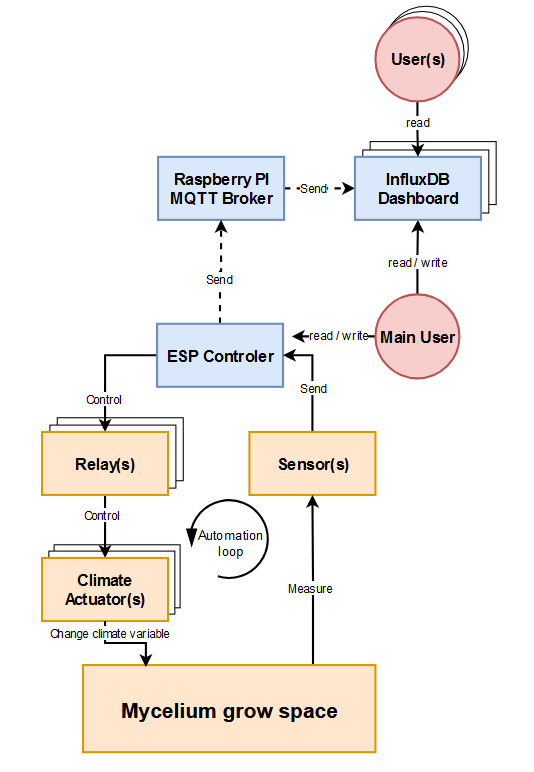
\includegraphics{images/diagMyceliummachine.png}
%     \caption{System design representation}
%     \label{fig:blasttrash}
% \end{figure} 

\section{Systems design}



\begin{figure}[h]
    \centering
    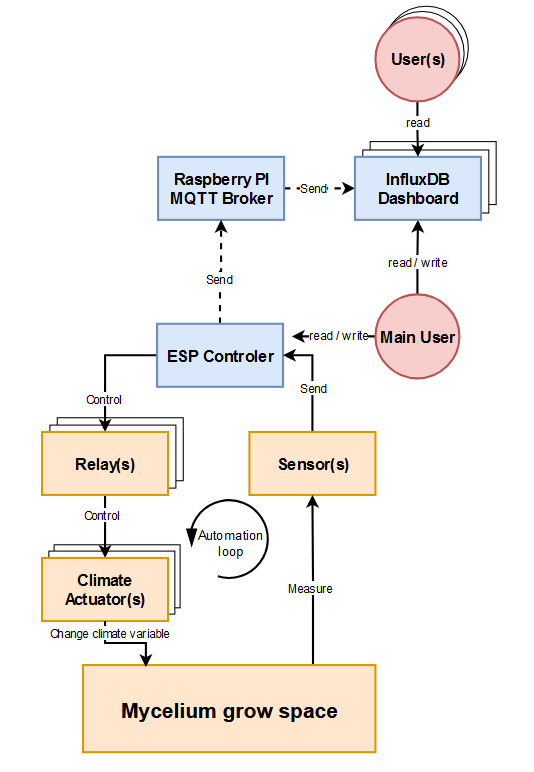
\includegraphics{images/diagMyceliummachine.png}
    \caption{System design representation}
    \label{fig:blasttrash}
\end{figure} 


\section{Manufacturing Processes \& Grow Theory}

\section{Contribution}

\subsection{Environment controlled}
\subsection{Modular environmental control}



\section{Result}
\subsection{Mechanical test}






